\section{Case Study}
\label{sec:case}
This case study presents the aggregation of multiple flexible DERs via coordinated operation: 75 DERs installed in a suburban residential area, which are all connected to the same feeder leading to a 10/0.4 kV transformer. The transformer is rated to a maximum power flow of 200 kVA, which is sufficient under the current load circumstances, but will be a constraint in the future.

This case study addresses a scenario with high electric-vehicle (EV) penetration, low photo-voltaic (PV) penetration and electric space heating in all households. Furthermore all DERs connected to the same LV feeder offer their flexibility to the same Aggregator. Then, the proposed performance index for service provision is evaluated for two different aggregation control algorithms: Centralized soft Model Predictive Control (C-MPC) and Distributed soft Model Predictive Control (D-MPC).

\subsection{The reference case: without units coordination}
In this section we make a scenario hypothesis for year 2050 regarding PV and EV penetration in a distribution feeder in a rural area and present simulation results. The following units are connected to the LV transformer:
\begin{itemize}
\item 40 buildings with electric climate control: resistive space heating with maximum load of 10 kW and air conditioning with a maximum load of 5 kW.
\item 20 large EVs, with a battery size of 25 kWh, 11 kW.
\item 10 small EVs, with a battery size of 14 kWh, 3.3 kW.
\item 5 PV (polycrystalline) installations of 6 kW rated power each.
%\item 5 Li-On support batteries for local energy storage: 10 kWh, 2 kW each (95\% round trip efficiency). 
\end{itemize} 

The PV installations provide forecasts of the production for one day ahead. To simulate uncertainty in the forecasts, Gaussian noise has been added to real data of PV production according to:
\begin{equation}
	{P_{PV-F,t}} = {P_{PV-T,t}} + {v_t},\quad {v_t} \sim N\left( {0,\alpha  \sqrt {{P_{PV-T,t}}} } \right)\label{eq:pvprod}
\end{equation}
where $P_{PV-F,t}$ is the forecasted PV power production at time $t$, and $P_{PV-T,t}$ is the actual power production at time $t$ (from historical data). The term $\alpha$ is an uncertainty factor, which defines the variance of the noise as a percentage of the actual PV production, e.g. $\alpha = 0.1$ corresponds to a $10\%$ forecast error. Uncertainty in solar radiation and ambient temperature are modeled in the same way. The actual power production time-series used in this case covers the same days as \cite{costanzo2013coordination}.

The load related to households is divided into climate control (flexible load) and everything else (non-flexible load). The building climate control is operated on MPC basis for minimum deviation from the temperature set point. Regarding the non flexible household loads, a five-day (one-hour-sampled) profile of the non-flexible load of 40 households is depicted in Fig.~\ref{fig:nonflexible}.

\begin{figure}[t]  
	\centering
	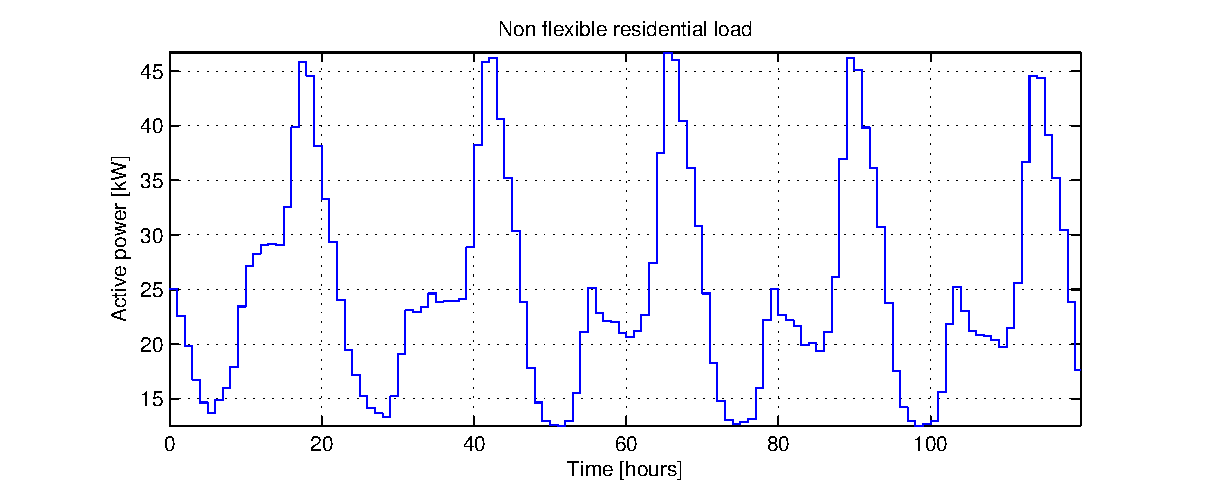
\includegraphics[width=\textwidth]{isgt2014/nonflexload.eps}
	\caption{The non-flexible load of the households under the transformer. The sample is statistically representative of Danish households.}\label{fig:nonflexible}
\end{figure}

The EVs leave the charging station at a uniform randomly distributed time between 6:00  and 8:00, and are plugged again at a uniform, randomly distributed time between 16:00 and 18:00. The EVs operate on dumb charging, i.e. they try to fully charge as soon as they are connected to the grid.  %The energy price is the same for all the units within the same cluster.
By running a simulation of the described scenario without units coordination, the results shown in Fig.~\ref{fig:referencecase} are obtained.

\begin{figure}[t]  
	\centering
	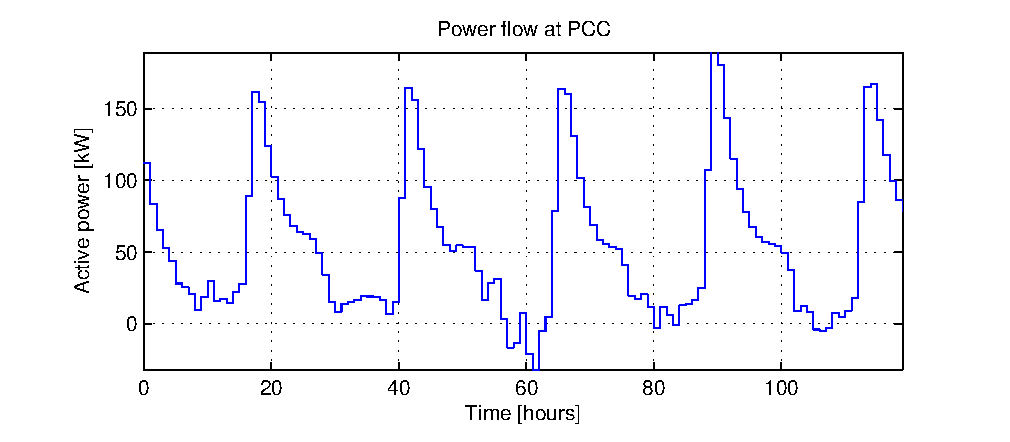
\includegraphics[width=\textwidth]{isgt2014/referencecase.eps}
	\caption{Aggregated power flow at the point of common coupling for the reference case units without coordination: Demand Response based on day-ahead energy price.}\label{fig:referencecase}
\end{figure}

EVs operating on dumb charging can cause peak consumption up to 190 kW at the point of common coupling (PCC). Given that the transformer capacity is 200 kW and it is customary to reserve 30\% of the transformer capacity for emergency operations \cite{Engel}, the DSO aims at keeping the load below 140 kW and limiting the inverse power flow at the substation. Thus, the DSO can sign a contract for PowerMax service (see Sec.~\ref{sub:example}) with an Aggregator which, at any time, operates Demand Response via Direct Load Control (DLC)~\cite{kosek2013overview} in order to limit the power flow at the transformer. The maximum capacity available at the transformer is therefore 140 kW for direct power flow and -10 kW for inverse power flow.

The rest of this section presents the C-MPC and D-MPC formulations. For the formulation of the mathematical models we refer to~\cite{6345063} for the battery model and to~\cite{Bacher20111511} for the building space heating model (modified, as proposed in~\cite{costanzo2013coordination}). For the modeling of the services, we apply the method described in Sec.\ref{sub:modelcalc}. A discussion on the simulation results concludes this section.
\subsection{The Centralized Model Predictive Control scheme}
\begin{figure}[t]  
	\centering
	\subfloat[The setup of the Centralized MPC scheme.]{\includegraphics[width=1.0\textwidth]{isgt2014/centralized.eps}\label{fig:centralized}}
\\
\subfloat[The setup of the DMPC scheme as seen in \cite{costanzo2013coordination}.]{\includegraphics[width=1.0\textwidth]{isgt2014/blackboard.eps}%
\label{fig:blackboard}}
\caption{The setup of the two Aggregation algorithms to be compared.}\label{fig:systemsetup}
\end{figure}
In this scheme the Aggregator contains the control algorithm to centrally manage all the units in its portfolio (Fig.~\ref{fig:systemsetup}(a)). Since the Aggregator optimizes its portfolio's consumption through MPC, it has detailed knowledge of the state and dynamics underneath.
The units portfolio is the same as of the reference case. The C-MPC control problem is formulated as quadratic optimization with soft constraints (as seen in e.g. \cite{prasath2009a}):
{%\footnotesize
{\begin{subequations}\label{Eq: building_MPC}
\begin{align}
& \min\limits_{u_t,\vartheta_t} \; {J} = \sum\limits_{t = 1}^N {\left[ {\left\| {y_{t} - r_t} \right\|_Q^2} + {\rho}\vartheta_t + \psi \gamma_t \right]} \label{Eq: building_MPC_objective}\\
& subject \; to: \nonumber \\
& x_{t + 1} = Ax_t + B u_t + Ed_t\label{Eq: building_MPC_constraint1}\\
& y_t = {C}x_t +Du_t \label{Eq: building_MPC_constraint2}\\
& u_{\min ,t} \le u_t \le u_{\max ,t} \label{Eq: building_MPC_constraint3}\\
& y_{\min ,t} - \gamma_t \le y_{t} \le y_{\max ,t} + \gamma_t \label{Eq: building_MPC_constraint4}\\
& {PCC_{\min ,t}} - \vartheta _t \le u_t \le {PCC_{\max ,t}} + \vartheta _t \label{Eq: building_MPC_constraint5}\\
& \vartheta_t,\gamma_t \ge 0 \label{Eq: building_MPC_constraint6}
%& \gamma_t \ge 0 \label{Eq: building_MPC_constraint7}
\end{align}
\end{subequations}}}
where $r_t$ and $y_t$ are the output reference and system outputs (internal house temperature and battery state of charge) respectively over the prediction horizon $t=1..N$, $\psi$ is the weight for output soft constraints, with $\gamma$ being the corresponding slack variable, and $\rho$ penalizes the \emph{power over max} defined in Eq.~\ref{Eq: building_MPC_constraint5}. Since this MPC controller is centralized, the state space system matrices in Eq.~\eqref{Eq: building_MPC_constraint1} and Eq.~\eqref{Eq: building_MPC_constraint2} are formed by block diagonal-adding each of the systems' respective matrices. With the set of units $\mathcal{S}=\{1..N\}$, it follows:
%
{ \begin{equation}
\begin{array}{l}
x = \left[ {\begin{array}{*{20}{c}}
{{x_1}}\\
{{x_j}}
\end{array}} \right],u = \left[ {\begin{array}{*{20}{c}}
{{u_1}}\\
{{u_j}}
\end{array}} \right],d = \left[ {\begin{array}{*{20}{c}}
{{d_1}}\\
{{d_j}}
\end{array}} \right],y = \left[ {\begin{array}{*{20}{c}}
{{y_1}}\\
{{y_j}}
\end{array}} \right]\\
\\
A = \left[ {\begin{array}{*{20}{c}}
{{A_1}}&0\\
0&{{A_j}}
\end{array}} \right],\quad B = \left[ {\begin{array}{*{20}{c}}
{{B_1}}&0\\
0&{{B_j}}
\end{array}} \right]\\
\\
C = \left[ {\begin{array}{*{20}{c}}
{{C_1}}&0\\
0&{{C_j}}
\end{array}} \right],\quad D = \left[ {\begin{array}{*{20}{c}}
{{D_1}}&0\\
0&{{D_j}}
\end{array}} \right]\\
\\
E = \left[ {\begin{array}{*{20}{c}}
{{E_1}}&0\\
0&{{E_j}}
\end{array}} \right],\quad \vartheta  = \left[ {\begin{array}{*{20}{c}}
{{\vartheta _1}}\\
{{\vartheta _j}}
\end{array}} \right],\gamma  = \left[ {\begin{array}{*{20}{c}}
{{\gamma _1}}\\
{{\gamma _j}}
\end{array}} \right]
\end{array}
\end{equation}}
%\normalsize
where the index $j \in \mathcal{S}$ and the system in Eq.~\eqref{Eq: building_MPC_constraint1} and Eq.~\eqref{Eq: building_MPC_constraint2} is extended with all the units belonging to the set $\mathcal{S}$.
\subsection{The Distributed Model Predictive Control scheme}
%The computational effort for solving centralized MPC problems generally grows at a super-linear rate with the number of state variables involved. The exact order is problem-specific and depends on the coupling between the state variables as well as the chosen solving method. Decomposing the C-MPC problem into smaller MPC sub-problems that can be solved independently and locally at the unit level helps in solving the curse of dimensionality. Convergence towards the overall goal is then achieved through a blackboard coordination mechanism, which ensures data exchange between the individual solvers.
In the D-MPC formulation, units within the same cluster retrieve the power plans of the other units, compute their own plan (over a prediction horizon) accordingly and publish it on a blackboard. Note that in this case study, in contrast to what has been proposed in~\cite{costanzo2013coordination}, the unit controllers have soft constraints on the outputs (temperature for buildings and State of Charge (SOC) for batteries and EVs). In this algorithm, as soon as the units publish their consumption plan, the available power at the PCC decreases in such a way that the subsequent units communicating with the blackboard tend to adjust their plan accordingly. After a negotiation period the units are entitled to operate according to the power plan that has been published in the blackboard for the next time frame. Figure~\ref{fig:systemsetup}(b) shows the configuration for the D-MPC. This is an example of transactional control \cite{kosek2013overview}, where the unit power consumption is negotiated.
\subsection{Comparison and discussion of results} \label{sub:comparison}
Certain assumptions have been made with regards to controllers:

%\begin{itemize}
The EVs are preferably kept operating in the range $SOC = [0.2,0.9]$ due to battery life concerns\cite{6345063}, although it is possible to operate in $SOC=[0.0,1.0]$.
The comfort band for the households lies in the band $T_{ref}=22{}^{\circ} C \pm 1{}^{\circ} C $. The concept of non-delivery is not used in the asset-management services, but the absolute boundaries for user-comfort bands lie on $T_{ref}=22{}^{\circ} C \pm 1.5{}^{\circ} C $.

The required PowerMax service is of $P_M = 90kW $ each day in the periods of 16:30 to 20:30.
The time sampling of the simulation is of 15 minutes and the power plans are computed for a horizon of 23 hours (i.e. the MPC prediction horizon).
%\item The EVs are not available during the day, when they are used for transport, and in these periods the MPC for the EV is inactive.
The EVs are not capable of providing Vehicle-to-Grid (V2G) services, i.e. EVs only charge.

%\end{itemize}
These assumptions lead to the results presented Figs.~\ref{fig:dmpcsimres}-\ref{fig:pccsimres} and Tables \ref{tab:comparison}-\ref{tab:days}.
The following conclusions can be made:

1) from Figs.~\ref{fig:dmpcsimres} and \ref{fig:cmpcsimres} it can be seen that both controllers are quite good at staying within the QoS limits of the DSO and EV owners, which can be seen in the fact that none of the controllers have non-delivery and $\eta$ is small. It is clear that the value of $\eta$ comes from the behavior of the household heating, where the C-MPC delivers a better quality service to end users than the D-MPC, although it might not be obvious from the figures. % Also, from Fig.~\ref{fig:pccsimres}, it is clear that the PowerMax service is delivered at all times.

2) controller performance is sensitive to prediction uncertainties, as can be seen in the varying values of $\eta$ depending on the uncertainty $\alpha$ (see Eq.~\eqref{eq:pvprod}), which is shown in Table~\ref{tab:comparison}.
	%\item By changing some of the different weights on the controllers, e.g. prioritizing the upwards service versus the downwards service, leads to different results it $\eta$ (this is not shown in the figures).

3) in terms of service provision, the C-MPC outperforms the D-MPC. This arises from the fact that the C-MPC has absolute control of all units and determines a global optimum.

4) due to the behavior difference between the local EV controllers in the D-MPC scheme, and the behavior of the C-MPC, the power consumption of the EV is very different (compare Fig.~\ref{fig:dmpcsimres}(b) and Fig.~\ref{fig:cmpcsimres}(b)). This also leads to a vast difference in the power flow at PCC (see Fig.~\ref{fig:pccsimres}).

5) from the values in Table~\ref{tab:days}, it can be seen that the values of $\eta$ are in the same order of magnitude when simulations are done for varying numbers of days. This is caused by the normalization of $J_{act}(N)$ over time (reflected in $J_{max}(N)$). This means $\eta$ evaluates the aggregation algorithm taking service provision time into account, and gives an overall assessment of the algorithm, dependent on the length of time the Aggregator must sustain the service provision. %An error in provision of a specific size will have less impact on $\eta$ if the service time is long. This makes sense since an error  

\begin{figure}[!t]
\centering
\subfloat[Households temperatures]{\includegraphics[width=1.0\textwidth]{isgt2014/DMPCalpha01/building2.eps}%
\label{fig:dmpchouse}}
\\
\subfloat[EV State of Charge]{\includegraphics[width=1.0\textwidth]{isgt2014/DMPCalpha01/EVs.eps}%
\label{fig:dmpcev}}
\caption{Simulation results for the D-MPC with $\alpha=0.1$}
\label{fig:dmpcsimres}
\end{figure}

\begin{figure}[!t]
\centering
\subfloat[Households temperatures]{\includegraphics[width=1.0\textwidth]{isgt2014/CMPCalpha01/buildings.eps}%
\label{fig:cmpchouse}}
\\
\subfloat[EV State of Charge]{\includegraphics[width=1.0\textwidth]{isgt2014/CMPCalpha01/EVs.eps}%
\label{fig:cmpcev}}
\centering
\caption{Simulation results for the C-MPC with $\alpha=0.1$}
\label{fig:cmpcsimres}
\end{figure}

\begin{figure}[!t]
\centering{\subfloat[Total power load for C-MPC]{\includegraphics[width=0.5\textwidth]{isgt2014/CMPCalpha01/PCC.eps}%
\label{cmpcpcc}}
\subfloat[Total power load for D-MPC]{\includegraphics[width=0.5\textwidth]{isgt2014/DMPCalpha01/PCC.eps}%
\label{dmpcpcc}}}
\centering
\caption{Power load at Point of Common Coupling for the controllable and non-controllable loads}
\label{fig:pccsimres}
\end{figure}

% increase table row spacing, adjust to taste
%\renewcommand{\arraystretch}{2.3}
%if using array.sty, it might be a good idea to tweak the value of
% \extrarowheight as needed to properly center the text within the cells
\begin{table}
\caption{Results of three-day simulation}\label{tab:comparison}
\centering
% Some packages, such as MDW tools, offer better commands for making tables
% than the plain LaTeX2e tabular which is used here.
\begin{tabular}{c|c c c c}
\hline
&\multicolumn{2}{c}{D-MPC} & \multicolumn{2}{c}{C-MPC} \\
\hline
$\alpha$ & 0.1 &0.2&0.1&0.2\\
NDC&0 &0 &0 &0\\
$\eta$&0.0075 &0.0160&0.0054&0.0153\\
\hline
\end{tabular}
\end{table}

\begin{table}
	\caption{D-MPC Performance over different simulation lengths}\label{tab:days}
	\centering
\begin{tabular}{c|c c c c c}
\hline
Days simulated & 1 & 2 & 3 & 4 & 5 \\
$\eta$ &0.0013&0.0018 &0.0082&0.0052&0.0062\\
\hline
\end{tabular}
\end{table}
